\xchapter{Background}{} \label{chapter:background}

In this section, we briefly introduce main concepts relevant to understand the developed work. 

\section{Public Communication of Emergencies} Emergencies are defined as critical situations caused by incidents, natural or man-made, that require measures to be taken immediately to reduce their adverse consequences to life and property \cite{dha1992internationally}. The adverse and therefore undesired consequences of an emergency give rise to a crisis.
An emergency comprises a random and totally unexpected event. However, it presents patterns that can help communicators anticipate problems and be able to give an immediate response \cite{cdc2014}, hopefully avoiding a crisis.

However, emergency and crisis are used as synonym in the field of public communication. In this context, the term "crisis communication" is used with two meanings. The first one refers to the communication among organisations involved in the emergency management. The second one is related to the need of the emergency management to inform/alert the public about the emergency \cite{cdc2014}. The last definition is the one that best fits the scope of our research.

This chapter describes the main characteristics of public communication in emergencies/crises. Additionally, it presents concepts and best practices on Crisis and Emergency Risk Communication.

\subsection{Crisis and Emergency Risk Communication}

One key aspect of emergency management is communication, which can help people and organisations to handle the emergency situation in a better way. The challenge of this activity is to establish a good strategy for communication with the partners that should be informed. A simple definition for Crisis and Emergency Risk Communication (CERC) is: a set of principles that aim to guide emergency managers to know what to say, when to say, how to tell and thus preserve or win the public's confidence during a crisis \cite{cdc2014}.

After analysing a set of studies in this field, we selected the CERC study \cite{cdc2014} to provide detailed information on crisis and emergency communication. CERC is a general theoretical framework developed by Centres for Disease Control and Prevention (CDC) of the United States of America. Its basic principle of communication is: be first, be right, and be credible.
Two additional concepts are essential to understand the CERC principles: Crisis communication and Risk communication.

\begin{itemize}
   \item \textbf{Crisis Communication:} it refers to communication activities of an organisation that is facing a crisis. However, the term may be associated either with the management of emergency or the effort involved in the task of alerting and keeping the public informed about an incident \cite{cdc2014}. 
   \item \textbf{Risk Communication:} it comprises the “information exchange about health risks caused by environmental, industrial, or agricultural, processes, policies, or products among individuals, groups, and institutions” \cite{glik2007}.
 \end{itemize}

CERC arises from the application of risk communication principles in crisis communication, i.e., it incorporates communications about possible risk factors into the communication of the crisis evolution \cite{reynolds2005}.

\subsection{The CERC Lifecycle}  \label{cercPhase}
Despite a crisis being a random and totally unexpected event \cite{cdc2014}, it presents patterns that support communicators to anticipate problems and give immediate response. A crisis can be divided into the following phases: pre-crisis, initial, maintenance, resolution and evaluation \cite{cdc2014} \cite{reynolds2005}.
 
 
\textbf{\\Pre-crisis phase\\}
In this phase, the goal is educational and it aims at preparing the public to know how to behave in an emergency situation. In this phase, it is important to test the public communication systems, detecting potential problems and ensuring their full operation in real crisis situations.

\textbf{\\Initial phase\\}
In the initial phase, the priority is to inform the general public and the affected people about the occurrence of the incident \cite{reynolds2005}. This information must be passed quickly, but ensuring its reliability. More specifically, the message content in the initial phase should have the following attributes: be simple, credible, accurate, consistent, and delivered on time \cite{cdc2014}.

The purpose of communication is to ensure:

\begin{itemize}
   \item the empathy and reassurance of the public, reducing emotional turmoil;
   \item the understanding of the responsibilities of the organisations involved in the crisis;
   \item that the public knows where they can get more information.
 \end{itemize}
 
 In both application scenarios of our research, incidents at industrial parks and at large-scale events, this phase is associated to the period between the arrival of the first reports of an incident at the command and control centre and the arrival of work forces at the place of the incident. The emergency status at the end of this phase is \textbf{"Being Controlled"}, as called by the emergency coordinators from industrial parks and large-scale events in the workshops that we carried out.
 
\textbf{\\Initial phase\\}
 
 Communication in the maintenance phase seeks to ensure that the public:
 
 \begin{itemize}
   \item understands the risks involved in the incident and how to prevent them;
   \item is instructed about misunderstandings or rumours;
   \item receives guidance on protective actions that should be taken;
   \item is aware of actions taken by emergency managers and workforces to control the incident.
   
 \end{itemize}
 
 
 This phase covers the period between the moment in which the workforces at the incident place start handling the incident (e.g., fighting the fire), which corresponds to the emergency status \textbf{“Being Controlled”}, and the moment in which they finish handling the incident per se, but they still need to take protective measures, which corresponds to the emergency status \textbf{“Under Control"}.
 
  \textbf{\\Resolution phase\\}
  
  In the resolution phase it is important that the communicator continues to provide information to the public about the incident, presenting the measures that are being taken to overdue the damages caused by the incident. At the end of this phase the status of the emergency is \textbf{“Finished”}.
  
  
  \textbf{\\Evaluation phase\\}
  
  The last phase starts after the crisis is finished. At this stage it is important that crisis managers analyse how the communication occurred during the crisis and propose actions to improve the process. During this phase, the documentation that reports the crisis and the lessons learned is elaborated. This phase start after the end of the emergency and, for this reason, is outside the scope of our research. 
  
\subsection{Steps of Crisis Response}

\begin{figure}[htb]
\begin{center}
  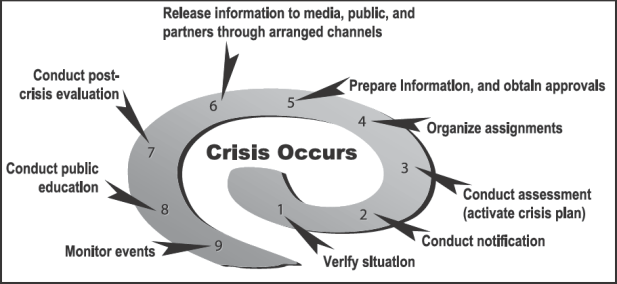
\includegraphics[scale=0.6]{images/CrisisSteps}
\caption{Steps of Crisis Response \cite{centers2006crisis}}
\label{fig:nineSteps}
\end{center}
\end{figure}

Usually, the initial moments of an emergency are considered the most chaotic. They are marked for the existence of uncertainty, panic and a great demand for information about the current situation, either for the emergency teams or for the external public affected directly or indirectly by its consequences. 

Faced with this critical situation, it is necessary that the crisis team promptly respond to the information needs of different publics. 

To help the crisis teams to effectively manage the most emergencies the CDC \cite{centers2006crisis} propose 9 generics communications steps to design a good crisis communication plan. The figure \ref{fig:nineSteps} shows each step proposed to crisis response.

\begin{enumerate}
   \item \textbf{Verify the Situation}: The first task for emergency response is the "situational awareness", i.e, get reliable information about the occurred facts from credible sources; 
   \item  \textbf{Conduct Notifications:} In the following, the crisis team needs to notify all partner (organisations and key people) involved in the crisis mitigation;
   \item  \textbf{Conduct Crisis Assessment:} The crisis team needs  to be continually updated about new information,  the severity of the situation, the target audience, and what information should be communicated;
   \item \textbf{Organise Assignments Quickly:} assign quickly, for your team and partners, of responsibilities, tasks and a consistent response to all communication needs; 
   \item \textbf{Prepare Information and Obtain Approvals:} Prepare Information and Obtain Approvals: is in this step, the crisis communication team will develop messages for public communication in a timely release;
   \item \textbf{Release Information through Prearranged Channels:} Select the target audience and the communication channels to disseminate rapidly the public communications. Prior to a crisis, is important that the crisis communication team identify the possible audience and the most appropriate communication channel for each;
   \item \textbf{Obtain Feedback and Conduct Crisis Evaluation:} Evaluate periodically the communication process during the crisis in order to detect possible communication problems. Feedback from key audience and media are a good way to make this evaluation;   
   \item \textbf{Conduct Public Education:} the period after the occurrence of a crisis is an opportunity to provide educational improvements on the population about the preparation for future crisis situations;   
   \item \textbf{Monitor Events:} Finally, is necessary observe the communication activities in social media, press, etc. to determine how to improve messages and the communication strategy. 
\end{enumerate}   

Some of these steps (Steps 2, 4, 8 and 9) are linked directly to the communication between organisations or people involved in the crisis management. This type of crisis communication is out of the scope of our research.

The step 7 and 9 relate to the monitoring and obtaining information from the repercussions generate by the crisis situation. This research is linked to the public communication of emergencies but is not related to the task of creation and disseminations of public communications.

The process to create and disseminate public communications can be described in 3 tasks: obtaining reliable information about the emergency, build appropriated messages for each target-audience and disseminate this messages, quickly, through multiple communication channels. These tasks are contained in the steps 1, 3, 5 and 6. The proposed computational model in this research was structured based on this steps.

 
  \subsection{Best Practices}
  
  Several studies have been conducted to propose good communication principles \cite{cdc2014} \cite{seeger2006best} \cite{goldfine2011best} \cite{glik2007} \cite{tinker2010} \cite{panamericanhealthorganization2009}.  Some of the principles are essential for effective communication with the public during an emergency:
  
  \begin{itemize}
   \item communicate repeatedly;
   \item be clear (use simple language and do not use technical terms, statistics or probabilities);
   \item communicate by different tools, media and communication channels (never trust on a single method of communication);
   \item transmit consistent information; and
   \item provide only relevant information.
   
 \end{itemize}
 
 The studies \cite{cdc2014} and \cite{cisvGuide} also indicate the basic information the crisis/emergency communicators need to know about an emergency situation:
 
 \begin{itemize}
   \item WHAT happened?
   \item WHERE did it happen?
   \item WHEN did it happen?
   \item WHO is involved?
   \item HOW did it happen?
   \item WHAT is currently being done?
      
 \end{itemize}
 
 About the content of the public messages, \cite{reynolds2007crisis} propose a set of good characteristics that those messages need to have. This principal is called “STARCC" and it maintains that the messages must be:
 
 \begin{itemize}
   \item Simple: Frightened people don’t want to hear big words
   \item Timely: Frightened people want information NOW
   \item Accurate: Frightened people won’t get nuances, so give it straight
   \item Relevant: Answer their questions and give action steps
   \item Credible: Empathy and openness are key to credibility
   \item Consistent: The slightest change in the message is upsetting and
dissected by all
      
 \end{itemize}

\section{Feature Modeling}

Software product line (SPL) \citep{malizia2010sema4a} is a software engineering method to abstract and represent the concept of variability in software that shares a set of similarities. Feature modelling is a compact visualization of different features of a SPL and its relationships. 

Feature modeling is one of the Feature-Oriented Domains Models presented by \cite{Kang1990}. Feature-Oriented Domain Analysis (FODA) is a domain analysis method proposed to support Software Reuse \citep{krueger1992software} at the functional and architectural levels. The main goal of this method is to manage the commonalities and variabilities within a product line.  

In the Feature Model, the features are arranged in a hierarchical structure. One feature (parent feature) can have sub-features (child features). 

The relationship between the parental feature and his sub-features can be of the type AND (all child must be selected); Alternative (only one sub-feature can be selected), or OR (one or more can be selected). 

The relationship between features is defined by two type of constraints: Implies and Excludes. When a feature needs one or more feature we have a relationship of Implies. When the opposite is true, the selection of one feature disables the selection of the other feature, we have the relationship of Excludes \citep{batory2005feature}.

We decided to model the variability of the emergency public communication domain do through feature modelling. We use this approach to guide the development of our variability based model in order to capable the addressing the different stakeholders’ needs in the most different scenarios of crisis/emergency.